\section{Model architecture and results} \label{sec:models}


\paragraph{Image Augmentation.}
The image augmentation  that we used in the models is the following:

\begin{itemize}
    \item \texttt{RandomFlip("horizontal\_and\_vertical")}
    \item \texttt{RandomRotation(0.1)}
    \item \texttt{RandomZoom(0.1)}
    \item \texttt{RandomCrop(45, 45)}
    \item \texttt{Resizing(50, 50)}
\end{itemize}


\subsection{Model with Optuna Results}

The architecture found by Optuna is summarized in 
Table~\ref{tab:optuna-best-model}. Apart from using redshift, 
the plasma temperature (\texttt{kT}) as an auxiliary input was found 
to be beneficial to the model by the optuna study. This model achieved 
a best validation MSE of $0.073$ 
and best negative log-likelihood (NLL) of $-0.08136$. The coverage 
within the predicted $1\sigma$ interval was $66.8\%$. These results 
are summarized visually in Figures~\ref{model:optuna_model_epochs} 
and~\ref{model:optuna_model_mass}.




\begin{table}[ht]
    \centering
    \caption{Summary of the best CNN architecture (Optuna-selected) used for mass regression, including auxiliary features redshift and temperature as inputs.}
    \label{tab:optuna-best-model}
    \begin{tabular}{|l|c|c|}
        \hline
        \textbf{Layer (type)} & \textbf{Output Shape} & \textbf{Param \#} \\
        \hline
        Input (image)                 & (None, 50, 50, 10)     & 0           \\
        Conv2D (32 filters, 5$\times$5)  & (None, 50, 50, 32)     & 8,032       \\
        Conv2D (32 filters, 2$\times$2)  & (None, 50, 50, 32)     & 4,128       \\
        Conv2D (128 filters, 2$\times$2) & (None, 50, 50, 128)    & 16,512      \\
        BatchNormalization              & (None, 50, 50, 128)    & 512         \\
        Flatten                         & (None, 320000)         & 0           \\
        Dense (64 units)                & (None, 64)             & 20,480,064  \\
        Dropout                         & (None, 64)             & 0           \\
        Dense (256 units)               & (None, 256)            & 16,640      \\
        Dropout                         & (None, 256)            & 0           \\
        Input (redshift)                & (None, 1)              & 0           \\
        Input (kT)                      & (None, 1)              & 0           \\
        Concatenate                     & (None, 258)            & 0           \\
        Dense (256 units)               & (None, 256)            & 66,304      \\
        Dense (2 units, output)         & (None, 2)              & 514         \\
        Lambda (final output)           & (None, 2)              & 0           \\
        \hline
        \textbf{Total}                  &                        & \textbf{20,592,706} \\
        \textbf{Trainable params}       &                        & \textbf{20,592,450} \\
        \textbf{Non-trainable params}   &                        & \textbf{256} \\
        \hline
    \end{tabular}
\end{table}


\begin{figure}[H]
    \centering
    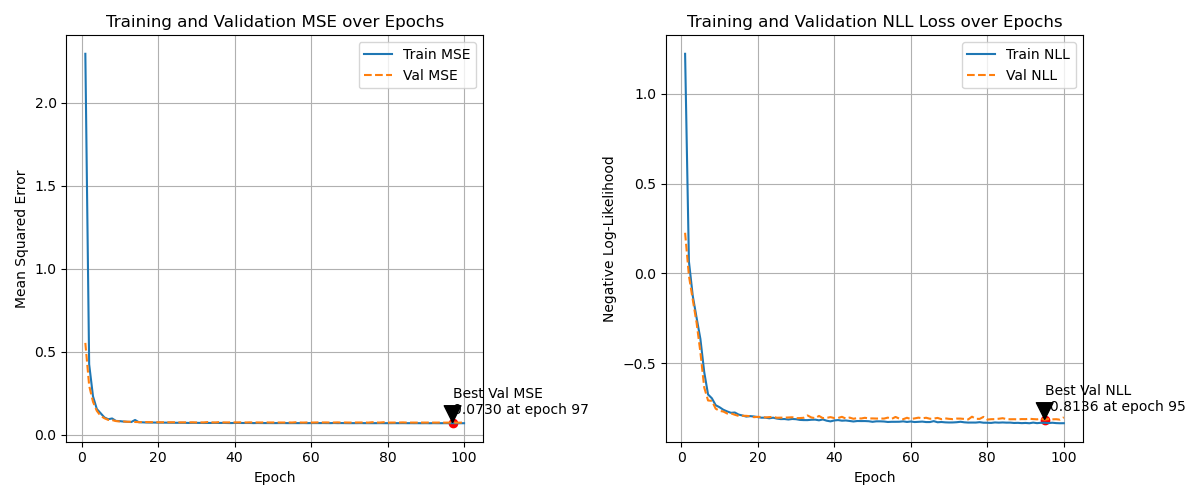
\includegraphics[width=0.8\linewidth]{chapters/models/optuna_model/metrics_vs_epoch.png}
    \caption{Training curves for MSE and NLL as functions of epoch.} \label{model:optuna_model_epochs}
\end{figure}

\begin{figure}[H]
    \centering
    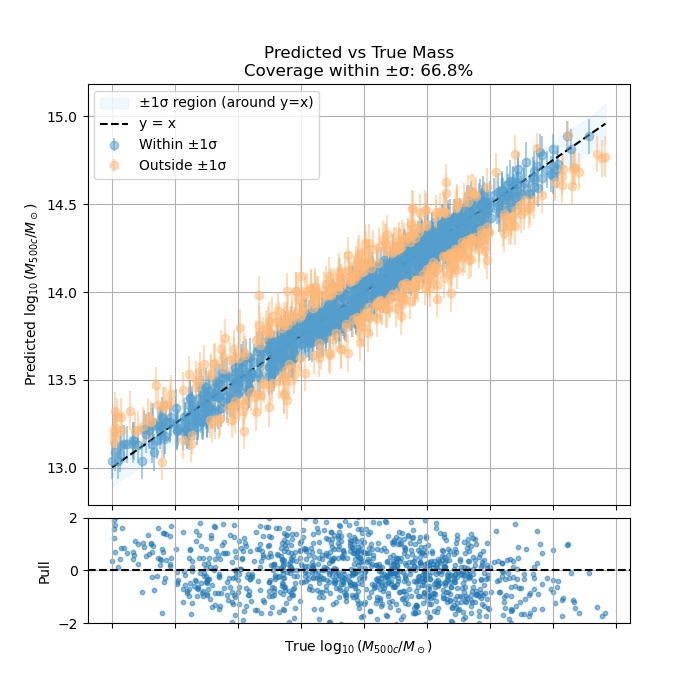
\includegraphics[width=0.8\linewidth]{chapters/models/optuna_model/mass_pred_test.png}
    \caption{Predicted vs true mass, $\pm1\sigma$ coverage, and pull distribution. } \label{model:optuna_model_mass}
\end{figure}



\subsection{Trial and Error model}
\label{sec:regularized-cnn-model}

This model achieved a best validation mean squared error (MSE) 
of $0.217$ and a best negative log-likelihood (NLL) of $0.0490$. 
The corresponding coverage within $\pm1\sigma$ was $90.3\%$, 
indicating improved uncertainty calibration compared to the Optuna-selected 
model. The key training curves and predictive performance are summarized 
in Figures~\ref{model:reg_model_epochs} and \ref{model:reg_model_mass}.

\begin{table}[ht]
    \centering
    \caption{Summary of the regularized CNN architecture with extensive use of BatchNorm and Dropout.}
    \label{tab:reg-cnn-model}
    \begin{tabular}{|l|c|c|}
        \hline
        \textbf{Layer (type)} & \textbf{Output Shape} & \textbf{Param \#} \\
        \hline
        Input (image)                 & (None, 50, 50, 10)     & 0           \\
        Conv2D (16 filters, 3$\times$3)  & (None, 50, 50, 16)     & 16,016      \\
        BatchNormalization              & (None, 50, 50, 16)     & 64          \\
        MaxPooling2D                    & (None, 25, 25, 16)     & 0           \\
        Conv2D (32 filters, 3$\times$3)  & (None, 25, 25, 32)     & 12,832      \\
        BatchNormalization              & (None, 25, 25, 32)     & 128         \\
        Conv2D (64 filters, 3$\times$3)  & (None, 25, 25, 64)     & 51,264      \\
        BatchNormalization              & (None, 25, 25, 64)     & 256         \\
        MaxPooling2D                    & (None, 12, 12, 64)     & 0           \\
        Conv2D (128 filters, 3$\times$3) & (None, 12, 12, 128)    & 32,896      \\
        BatchNormalization              & (None, 12, 12, 128)    & 512         \\
        MaxPooling2D                    & (None, 6, 6, 128)      & 0           \\
        Flatten                         & (None, 4608)           & 0           \\
        Dense (64 units)                & (None, 64)             & 294,976     \\
        BatchNormalization              & (None, 64)             & 256         \\
        Dropout                         & (None, 64)             & 0           \\
        Dense (32 units)                & (None, 32)             & 2,080       \\
        Dropout                         & (None, 32)             & 0           \\
        Input (redshift)                & (None, 1)              & 0           \\
        Input (kT)                      & (None, 1)              & 0           \\
        Concatenate                     & (None, 34)             & 0           \\
        Dense (16 units)                & (None, 16)             & 560         \\
        BatchNormalization              & (None, 16)             & 64          \\
        Dropout                         & (None, 16)             & 0           \\
        Dense (4 units)                 & (None, 4)              & 68          \\
        Dropout                         & (None, 4)              & 0           \\
        Dense (2 units, output)         & (None, 2)              & 10          \\
        Lambda (final output)           & (None, 2)              & 0           \\
        \hline
        \textbf{Total}                  &                        & \textbf{411,982} \\
        \textbf{Trainable params}       &                        & \textbf{411,342} \\
        \textbf{Non-trainable params}   &                        & \textbf{640} \\
        \hline
    \end{tabular}
\end{table}

\begin{figure}[H]
    \centering
    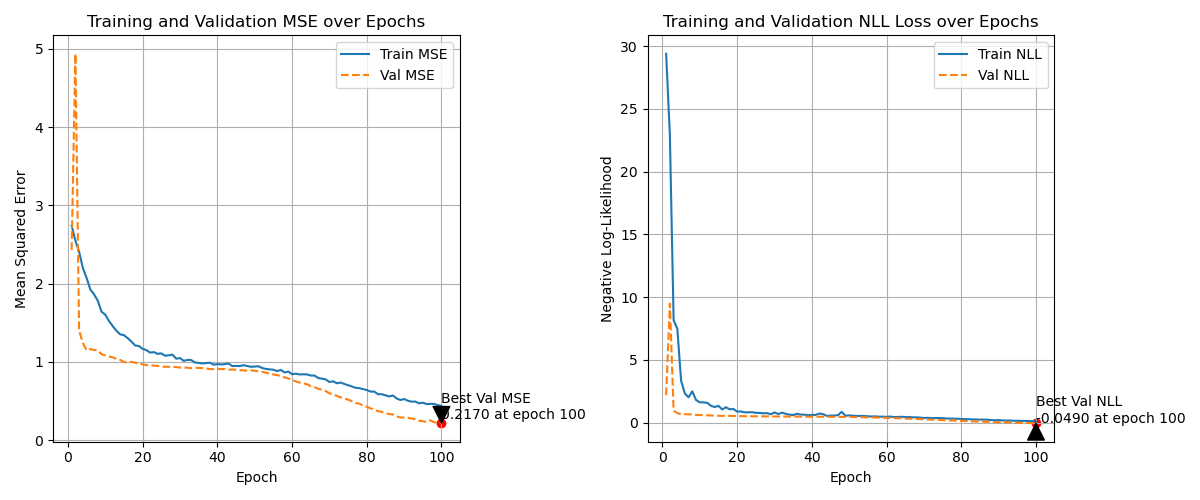
\includegraphics[width=0.8\linewidth]{chapters/models/other_model/metrics_vs_epoch.png}
    \caption{Training curves for MSE and NLL as functions of epoch.}
    \label{model:reg_model_epochs}
\end{figure}

\begin{figure}[H]
    \centering
    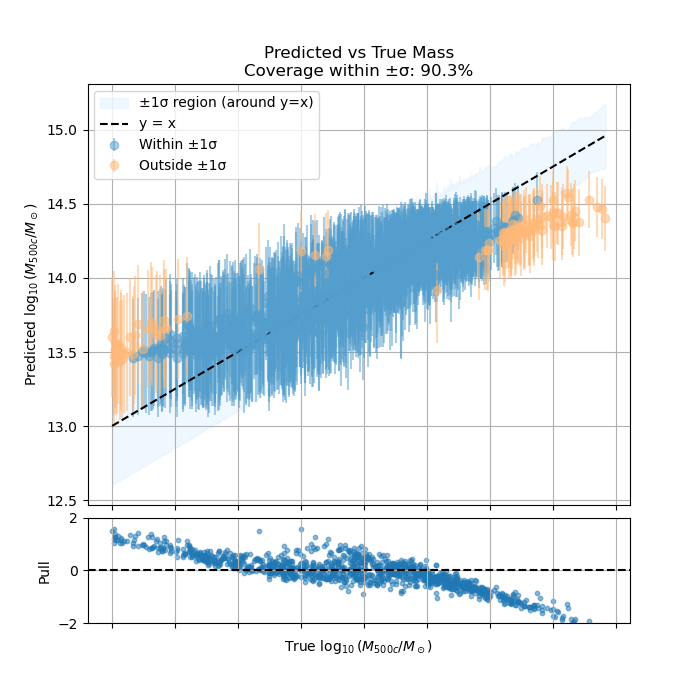
\includegraphics[width=0.8\linewidth]{chapters/models/other_model/mass_pred_test.png}
    \caption{Predicted vs true mass, $\pm1\sigma$ coverage, and pull distribution.}
    \label{model:reg_model_mass}
\end{figure}
